\subsection{Environmental Permit Application Process}
\label{subsec:coselog-wabo-process}
\textit{Environmental Permit Application Process} dataset originates from the "Configurable Services for Local Governments (CoSeLoG)" project \cite{van2011business} which investigates the similarities and dissimilarities between several processes of different municipalities in Netherlands. Dataset contains records of receiving phase for the building permit application process in 5 municipalities, which are comparable since activity labels in the different event logs refer to the same activities performed in five municipalities. In this dataset \cite{coselog-data}, there are 1214 cases and 2142 events with a variable distribution between event logs of municipalities and municipalities are used as organizational logs.

\begin{itemize}
  \item In \textit{Process Model Mining} stage, with 10 \% of noise threshold, high fitness values are achieved; however, some of the process models like Municipality \#4 and \#5 resulted with low appropriateness values. 
  \item In \textit{Performance Indicator Analysis} stage, after calculating the performance indicators, municipalities are clustered and three clusters are created: Municipality \#1 is located in the first cluster; Municipality \#2 and \#4 are located in the second cluster; and Municipality \#3 and \#5 are grouped in to the last cluster.
  \item In \textit{Mismatch Pattern Analysis} stage, it can be stated that as the similarity between process models of municipalities increases, number of mismatch patterns decreases for most of the cases. When further analyzed, it can be seen that Municipalities \#4 and \#5, which have significantly more complex process models compared to others, fail in spotting mismatch patterns under \textit{graph-edit similarity}.
  \item In \textit{Recommendation Generation} stage, for different threshold values, number of performance indicators that are performing better for the selected organization and spotted mismatch patterns are plotted in Figure~\ref{fig:coselog-wabo-recommendation-generation-analysis} for the thresholds of 25 \%, 50 \% and 75 \% since these are the breaking points. For instance, cluster of Municipality \#1 performs worse in 6 indicators with the difference of 25 \% and on average 5 mismatch patterns are listed for each performance indicator. When it is compared to the total mismatch patterns of Municipality \#1, which is 357, proposed approach helps significantly to the user for focusing performance improvement.
	\begin{figure}
		\centering
		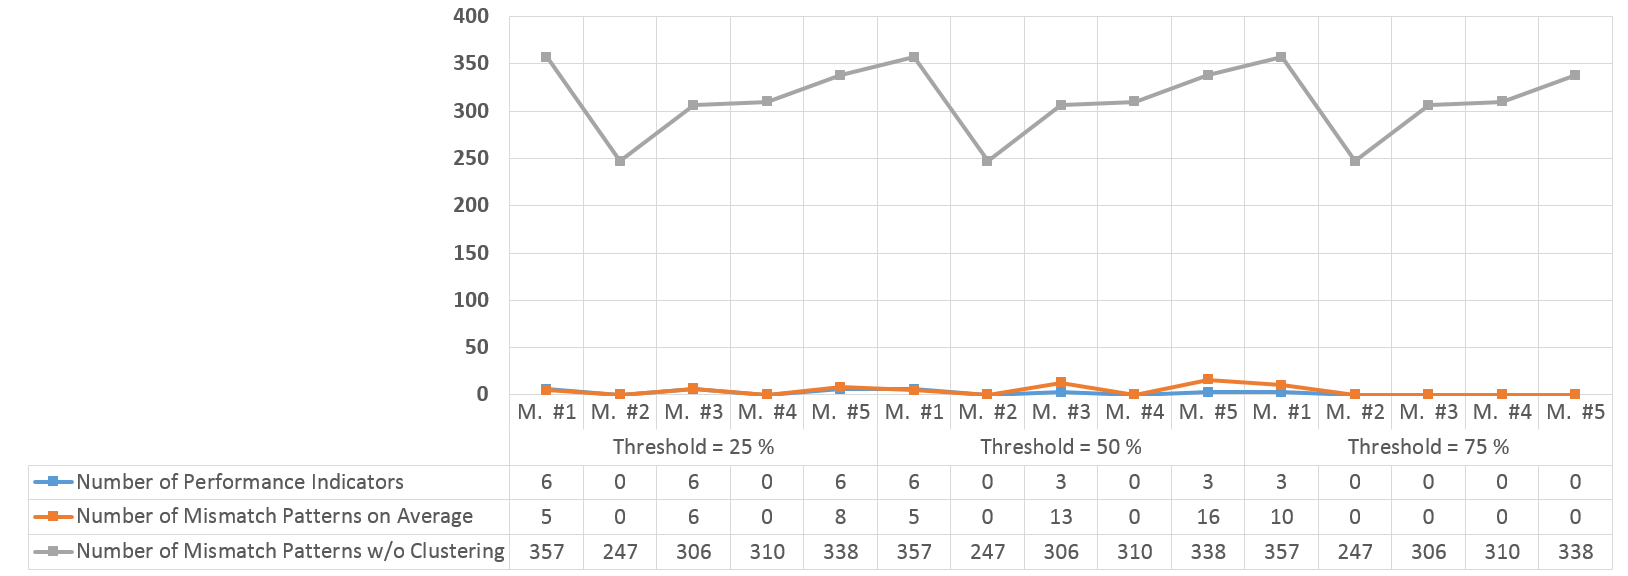
\includegraphics[width=\textwidth]{5_results_discussions/coselog-wabo/recommendation-generation-analysis-k3}
		\caption{Recommendation Generation analysis for Environmental Permit Application Process dataset (3 Clusters)}
	  \label{fig:coselog-wabo-recommendation-generation-analysis}
	\end{figure}
\end{itemize}
